% This is samplepaper.tex, a sample chapter demonstrating the
% LLNCS macro package for Springer Computer Science proceedings;
% Version 2.21 of 2022/01/12
%
\documentclass[runningheads]{llncs}
%
\usepackage[T1]{fontenc}
% T1 fonts will be used to generate the final print and online PDFs,
% so please use T1 fonts in your manuscript whenever possible.
% Other font encondings may result in incorrect characters.
%
\usepackage{graphicx}
% Used for displaying a sample figure. If possible, figure files should
% be included in EPS format.
%
% If you use the hyperref package, please uncomment the following two lines
% to display URLs in blue roman font according to Springer's eBook style:
%\usepackage{color}
%\renewcommand\UrlFont{\color{blue}\rmfamily}
%\urlstyle{rm}
%
\begin{document}
%
\title{New Schema Mechanisms to Implement Genetic Epistemology}
%
\titlerunning{Schema Mechanisms}
% If the paper title is too long for the running head, you can set
% an abbreviated paper title here
%
\author{Olivier L. Georgeon\inst{1}\orcidID{0000-0003-4883-8702} \and
Filipo Perotto\inst{2}\orcidID{1111-2222-3333-4444} \and
Third Author\inst{3}\orcidID{2222--3333-4444-5555}}
%
\authorrunning{O. Georgeon \& F. Perotto}
% First names are abbreviated in the running head.
% If there are more than two authors, 'et al.' is used.
%
\institute{UR CONFLUENCE: Sciences et Humanites (EA 1598), UCLy, France \email{ogeorgeon@univ-catholyon.fr}\\
	\and ONERA, France \email{filipo.perotto@onera.fr}
 \and
 }
%
\maketitle              % typeset the header of the contribution
%
\begin{abstract}
We review schema mechanisms as they have been used to account for a \textit{genetic} or \textit{constructivist} theory of learning.

\keywords{Schema mechanism  \and Genetic epistemology \and Constructivist learning.}
\end{abstract}
%
%
%
\section{Introduction}



\section{Genetic epistemology}

The notion of \textit{sensori-motor scheme} proposed by Piaget \cite{piaget_principles_1997}. 
Related to constructivist epistemology by \cite{glasersfeld_radical_1997}.


Piaget's genetic epistemology : 
``Knowledge does not originally arise either from a subject conscious of itself or from objects already constituted (from the subject's point of view) that would impose themselves on the subject. 
Knowledge results from interactions occurring halfway between the subject and the objects, and thus involving both, but due to a complete un-differentiation and not from exchanges between distinct forms.

If, at the beginning, there is neither a subject, in the epistemic sense of the term, nor objects, conceived as such, nor, above all, invariant instruments of exchange, then the initial problem of knowledge will be to construct such mediators. 
Starting from the contact zone between one's own body and the objects, these mediators will progressively engage more deeply in both complementary directions toward the exterior and the interior. 
It is from this dual progressive construction that the joint elaboration of both the subject and the objects depends.

The initial instrument of exchange is not perception, as rationalists too easily conceded to empiricism, but rather action itself, with its much greater plasticity. 
Certainly, perceptions play an essential role, but they partly depend on action as a whole, and some perceptual mechanisms that one might have thought to be innate or very primitive only emerge at a certain level of object construction.'' (translated from \cite{piaget_lepistemologie_2011}, p14-15)


Guerin and McKenzie \cite{guerin_survey_2013} proposed the graphical representation in Fig. \ref{fig:general}.

\begin{figure}
	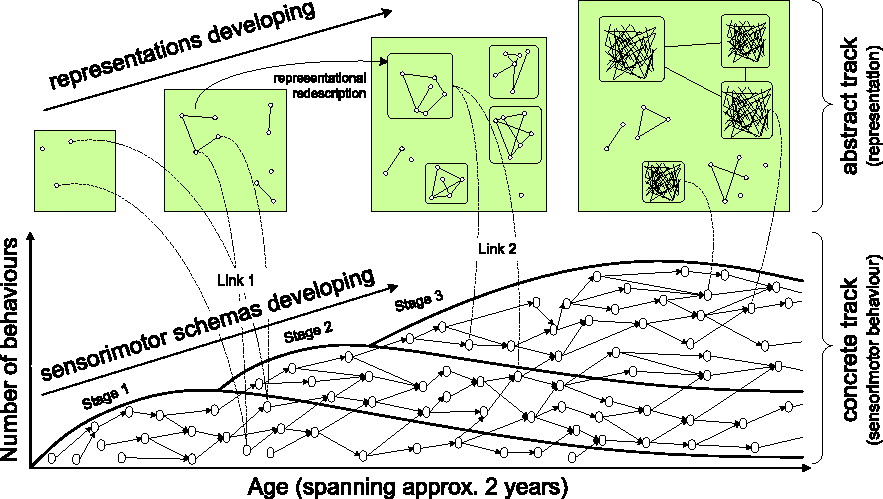
\includegraphics[width=\textwidth]{Figure_1_guerin.pdf}
	\caption{Conceptual diagram of infant development from \cite{guerin_survey_2013} Fig. 1.
	The lower (concrete) track shows a directed acyclic graph of sensorimotor schemas. 
	A node represents a newly created schema. 
	An edge has the meaning ``is a necessary precursor''. 
    Stage 1: behaviors without objects. 
    Stage 2: behaviors with single objects. 
    Stage 3: object-object behaviors. The schemas now involve relationship among objects, and locations and transforms within space.
    The higher (abstract) track represents representations of objects by schemas and physical properties influencing their interactions.} 
	\label{fig:general}
\end{figure}

Ziemke \cite{ziemke_construction_2001} examined how these views apply to robotics.


\section{Schema mechanisms}

Drescher \cite{drescher_made-up_1991} proposed the foundational schema mechanism by modeling schemas as depicted in Fig. \ref{fig:drescher}. 
A schema's context is satisfied when all the positively included items are On and all the negatively included items are Off. 
The activation is a schema consists of initiating its action. An activated schema is said to \textit{succeed} if its predicted results are all in fact obtained, and to \textit{fail} otherwise. The ratio of success and failure is called \textit{reliability} and is memorized for each schema.  
Schemas can be chained to achieve goals. 

\begin{figure}
	\centering
	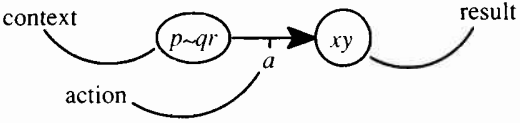
\includegraphics[width=0.6\textwidth]{Figure_2_schema_drescher.png}
	\caption{Schema from \cite{drescher_made-up_1991} Fig. 3.2.
	The schema noted $p \!\sim\! qr/a/xy$ asserts that if action $a$ is taken in the context where item $p$ is On, $q$ is Off, and $r$ is On then the items $x$ and $y$ will be turned On.} 
	\label{fig:drescher}
\end{figure}

\cite{drescher_made-up_1991}
\cite{chaput_constructivist_2004}
\cite{perotto_computational_nodate} 
\cite{guerin_piagetian_2008}
\cite{wang_new_2012}

\section{Benchmarks}

\begin{figure}
	\centering
	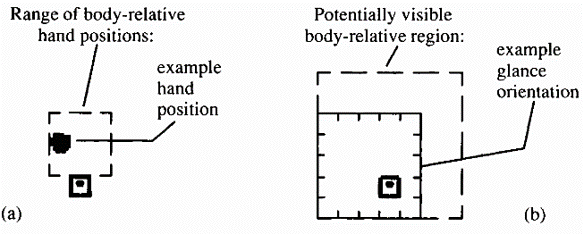
\includegraphics[width=0.6\textwidth]{Figure_drescher_expe.png}
	\caption{Drescher's experimental settings. From \cite{drescher_made-up_1991} Fig.6.1 ``Hand and glance ranges''.} 
	\label{fig:drescher2}
\end{figure}



\section{Autocatalytic enactive learning}

Bettoni  has criticized Drescher's schema mechanism in stating that ``Drescher's Constructivism is not Piaget's Constructivism, mainly because of its tacit acceptance of \textit{cognitive dogmatism}'' (\cite{bettoni_made-up_1993}, p. 6).
Bettoni describes cognitive dogmatism as taking for granted that ``patterns and structures of objects, attributes, relations, etc. [...] be as much as possible true copies of 'original' objects, attributes, relations etc. in the world'' (\cite{bettoni_made-up_1993}, p. 1).
Indeed, theories of enaction as well as of radical constructivism have insisted that we should not take the sensory signals as representational items of an alleged reality. 


The game of Mastermind provides an emblematic example in which the observation is not representational. 
Player 2 attempts to infer a hidden combination of colored pegs (``hidden state'') by proposing guesses (``actions''), which Player 1 responds to with feedback pegs (``observation''). Black pegs indicate a correct color in the correct position, while white pegs indicate a correct color in the wrong position.
Since the observation depends on the action, there exist no function or stochastic distribution that map the state to the observation. 
The absence of such function or distribution is expressed in cognitive terms by that the observation is not ``representational'' of the state.

Software to play mastermind have been proposed using diverse techniques such as entropy measure and evolutionary algorithms \cite{cotta_entropy-driven_2010}.
They, however require that the semantics of the feedback is known beforehand. 
The radical constructivist Mastermind analogy likens a general learner to someone playing a giant game of mastermind where they start with no knowledge of the hidden combination and even the semantics of actions and feedback.
The player may never find the hidden combination but may find a \textit{knowledge niche} in which to survive for some time.

Most schema mechanisms have been tested in settings in which the sensory signal is representational.
The fact that they have not been tested with non-representational sensory data does not mean that they would not work or could not be adapted to such settings. 

Georgeon and Ritter \cite{georgeon_intrinsically-motivated_2012} proposed an experimental settings where the sensory data is feedback from action rather than beeing representational. 
Fig. \ref{fig:agent8} illustrates the learning process that occurs in such settings. 

\begin{figure}
	\centering
	\includegraphics[width=1.0\textwidth]{Figure_3_agent8.pdf}
	\caption{Autocatatalytic enactive schema learning and selection.
	Schemas are nested tuples: (pre-schema, decision, post-schema).
	Over time, new decisions and new schemas are learned from the bottom up. 
	Recently enacted schemas (in gray) activate the previously-learned higher-level schema whose pre-schema they match.
	Activated schemas propose their post-schemas with a proclivity value calculated from the activation weight and the expected valence.
	The schema with the highest proclivity is selected to try to enact.} 
	\label{fig:agent8}
\end{figure}

A schema is recorded as tuple (pre-condition, decision, post-condition), similar to Drescher's schemas.
The pre-condition and post-condition, however, are not a representational description of the agent's situation but are just other schemas. 
The schemas are learned from the bottom up and nested hierarchically, with higher-level schemas made of a sequence of two previously-learned lower-level schemas. 
The system is initialized with a predefined set of primitive schemas that define the agent's basic possibilities of interaction. 
In a robot, primitive schemas are hard-coded control loops involving actuators end sensory feedback. 

At the end of time step $t$, the agent records or reinforces the schemas: 
\begin{itemize}
	\item[$\bullet$] $(i_{t-2}, d_{t-1}, i_{t-1})$
	\item[$\bullet$] $((i_{t-3}, d_{t-2}, i_{t-2}), d_{t-1}, i_{t-1})$
	\item[$\bullet$] $(i_{t-3}, d^2, (i_{t-2}, d_{t-1}, i_{t-1}))$
	\item[$\bullet$] $((i_{t-4}, d_{t-3}, i_{t-3}), d^2, (i_{t-2}, d_{t-1}, i_{t-1}))$
\end{itemize}

If it does not yet exist, the new decision $d^2$ is constructed different from the decision $d_{t-2}$ that was actually made at time $t-2$. 
for example, if the agent made decision $d_{t-2} = a0$ and enacted interaction $i_{t-2}=i00$, and then made decision $d_{t-1} = a0$, and enacted interaction $i_{t-1}=i01$, the agent learns the new decision $d^2=i00a0$ consisting of trying to enact the interaction $i_t=i00$ and then do action $a_{t+1}=a0$. 
When decision $d^2$ has been selected and successfully enacted, the mechanism learns higher-level schemas on top of it. 
The rate of schema construction being constant, the number of schemas grows linearly with time. 
Older and unused schemas can be forgotten.

Notably is not targeted at reaching a predefined goal. Since sensory data does not represent the environment's state, the agent cannot have a goal represented as an environment state. Instead, the agent's behavior is driven by the valence expectation of each decision. 
The calculation of expected valence may incorporate predefined preferences for some primitive schemas or different intrinsic motivation principles such as an estimation of information gained. 


\section{Conclusion}

The problem of abstraction. 


\begin{credits}
\subsubsection{\ackname} .

\subsubsection{\discintname}
The authors have no competing interests to declare that are
relevant to the content of this article.
\end{credits}
%
% ---- Bibliography ----
%
% BibTeX users should specify bibliography style 'splncs04'.
% References will then be sorted and formatted in the correct style.
%
\bibliographystyle{splncs04}
\bibliography{ConstructivistAI.bib}
%
\end{document}
